\documentclass[letterpaper,10pt]{article}

\usepackage{enumitem}
\usepackage{titling}
\usepackage{listings}
\usepackage{url}
\usepackage{hyperref}
\usepackage{setspace}
\usepackage{subfig}
\usepackage{sectsty}
\usepackage{pdfpages}
\usepackage{colortbl}
\usepackage{multirow}
\usepackage{multicol}
\usepackage{relsize}
\usepackage{amsmath}
\usepackage{wasysym}
\usepackage{fancyvrb}
\usepackage[yyyymmdd]{datetime}
\usepackage{amsmath,amssymb,amsthm,graphicx,xspace}
\usepackage[titlenotnumbered,noend,noline]{algorithm2e}
\usepackage[compact]{titlesec}
\usepackage{XCharter}
\usepackage[T1]{fontenc}
\usepackage[scaled]{beramono}
\usepackage[normalem]{ulem}
\usepackage{booktabs}
\usepackage{tikz}
\usetikzlibrary{arrows,automata,shapes,trees,matrix,chains,scopes,positioning,calc}
\tikzstyle{block} = [rectangle, draw, fill=blue!20,
text width=2.5em, text centered, rounded corners, minimum height=2em]
\tikzstyle{bw} = [rectangle, draw, fill=blue!20,
text width=4em, text centered, rounded corners, minimum height=2em]

\definecolor{namerow}{cmyk}{.40,.40,.40,.40}
\definecolor{namecol}{cmyk}{.40,.40,.40,.40}
\renewcommand{\dateseparator}{-}

\let\LaTeXtitle\title
\renewcommand{\title}[1]{\LaTeXtitle{\textsf{#1}}}

\lstset{basicstyle=\footnotesize\ttfamily,breaklines=true}

\newcommand{\handout}[5]{
	\noindent
	\begin{center}
		\framebox{
			\vbox{
				\hbox to 5.78in { {\bf SE 350: Operating Systems } \hfill #2 }
				\vspace{4mm}
				\hbox to 5.78in { {\Large \hfill #4  \hfill} }
				\vspace{2mm}
				\hbox to 5.78in { {\em #3 \hfill \today} }
			}
		}
	\end{center}
	\vspace*{4mm}
}

\newcommand{\lecture}[3]{\handout{#1}{#2}{#3}{Lecture#1}}
\newcommand{\tuple}[1]{\ensuremath{\left\langle #1 \right\rangle}\xspace}

\newcommand{\Rplus}{\protect\hspace{-.1em}\protect\raisebox{.35ex}{\smaller{\smaller\textbf{+}}}}
\newcommand{\Cpp}{\mbox{C\Rplus\Rplus}\xspace}


\addtolength{\oddsidemargin}{-1.000in}
\addtolength{\evensidemargin}{-0.500in}
\addtolength{\textwidth}{2.0in}
\addtolength{\topmargin}{-1.000in}
\addtolength{\textheight}{1.75in}
\addtolength{\parskip}{\baselineskip}
\setlength{\parindent}{0in}
\renewcommand{\baselinestretch}{1.5}
\newcommand{\term}{Winter 2023}
\newcommand{\termnumeric}{1231}

\singlespace


\begin{document}

\lecture{ 28 --- Scheduling: Idling, Priorities, Multiprocessor}{\term}{Jeff Zarnett}

\section*{Scheduling Algorithms, Continued}

Carrying on from last time, we will examine some more scheduling algorithms.

\subsection*{Highest Response Ratio Next}

We will introduce a new measure: normalized turnaround time. This is the ratio of the turnaround time (the time waiting plus the amount of time taken to execute) to the service time (the time it takes to execute). The relative amount of time waiting is somewhat more important; we can tolerate longer processes waiting a comparatively longer period of time. The goal, then, of the HRRN strategy, is to minimize not only the normalized turnaround time for each process, but to minimize the average over all processes~\cite{osi}.

The way to calculate the response ratio, $R$, is by the following formula: $\dfrac{w + s}{s}$ where $w$ is the waiting time and $s$ is the service time. The service time is, as always, a guess. When it is time to select the next process to run, choose the process with the highest $R$ value. A new process will have a value of 1.0 at the beginning, because it has spent no time waiting (yet). Thus it is not that likely to get selected.

Jobs with a small $s$, i.e., short jobs, are likely to get scheduled quickly, which is still a positive. In spite of this, the HRRN approach introduces something important we have not yet had: factoring in the age of the process. The term $w$ indicates how much time a process has spent waiting. Thus, a process that has spent a long time waiting will rise in priority, over time, until it gets a turn. So processes will not starve, because even a process that is expected to have a very long $s$ will eventually have a high enough $R$ due to the growth of $w$.

We still need to have some way of estimating $s$, which may or may not be simple guessing. 

\subsection*{Multilevel Queue (Feedback)}
For the most part, until now, we have treated processes more or less equally (except when we have taken the highest priority process). While it might seem very fair, it may not be ideal for a situation where processes behave differently. A desktop or laptop has many processes running, some of which are visible to the user (foreground, or interactive processes) and some of which are not (background and batch processes). We could then apply different scheduling algorithms to different types of process.

The multilevel queue takes the ready queue and breaks it up into several queues. A process can be in one (but only one) of the queues and it is assigned to the queue based on some attribute of the process (priority, memory needs, foreground/background, et cetera). The foreground queue, for example, could be scheduled by Round Robin, and the background by First-Come, First-Served~\cite{osc}.

When there are multiple queues, we also need a way of choosing which of the queues to take from next. The policy we choose depends on goals. We might say some queues have absolute priority over others (e.g., as in the earlier highest priority, period option), or we might have time slicing amongst the queues. This could be balanced evenly (rotate through each) or give more time slices to some queues at the expense of others.

An example of this was the CTSS (Compatible TimeSharing System) that ran on the IBM~7094. The CTSS designers decided that it was ideal to give CPU-Bound processes longer blocks of time to execute so they would not have to spend so much time swapping. They set up multiple queues. In the highest priority class, a process got 1 time slice; in the next one down, a process got 2 time slices; the third class meant 4 time slices, and so on. If a process ran up against the limit of a time slice (e.g., used the full 2 time slices), it was moved down a class. So it got a lower priority, but when it did get selected to run, it was able to run with a lower chance of being interrupted~\cite{mos}.

Like a few schemes, we have seen so far, this is a ratchet: a process can move down in the priority list, but there does not appear to be a way for it to move up. So a process that needed a lot of CPU early on was going to be punished ``forever''. The designers of the system assumed that if the user pressed the Enter key, it might be a sign the process was likely to become interactive (and therefore should move up in priority). Some genius user (there's always one), figured out that by pressing the enter button repeatedly, his long running processes would finish faster. This was a bit unfair; his processes got priority over the others. But things really broke down when this individual decided to be nice: he told all his friends. And suddenly everyone was doing it and the benefit of the system was lost~\cite{mos}.

This scheduling algorithm may also be referred to as \textit{feedback}. We do not have any information in advance about how long various processes will be. Instead of being concerned with how much CPU time will be used, which requires clairvoyance or guessing, we assign priority based on the amount of CPU time assigned so far. A process that has used a lot of CPU so far gets lower priority.

\subsection*{Guaranteed Scheduling}

And now for something completely different. The idea behind guaranteed scheduling is to promise the users something and then fulfill that promise. We could promise that if there are $n$ users, each gets an equal share (1/$n$) of the CPU time. Or with $m$ processes, each process gets 1/$m$ of the CPU time.

To make this happen, the system must keep track of how much CPU time each process has received since its creation. It then considers the how this value compares to the ideal (time since creation divided by $n$). If a process has a value of 0.5, it means it has had only half the CPU it ``should'' have received. If it has a value of 2.0, it has had double. So the scheduling algorithm is then to run the process with the lowest score, trying to keep all values as close to 1.0 as we can~\cite{mos}.

\subsection*{Lottery}

The lottery is a system to give predictable results with a simple implementation. The premise is that every process gets some number of ``lottery tickets'' for each resource (e.g., CPU). When a decision has to be made, a lottery ticket is selected at random. The process that holds that ticket gets that resource. This system provides some clarity; if a process has priority $p$, what does that mean? If a process has a fraction $f$ of the total tickets, then we can expect that process to get about $f$\% of the resource. When a process is created or terminates this may increase or decrease the number of tickets, or result in their redistribution~\cite{mos}. 

More important processes are given more tickets and have, therefore, a higher chance of winning. If there are 100 tickets outstanding, if a process has 25 of them, it has a 25\% chance of winning any given draw. To increase a process's chance of winning, give it more tickets. To decrease it, give it fewer. Unlike in the real lottery, though, there is always a winner. There are no ``unpurchased'' tickets and we can choose only a ticket that someone is holding.

Co-operating processes may be permitted to exchange tickets. A client that sends a request to a server might then give all its tickets to the server, increasing the chance the server gets the resources to run next~\cite{mos}.

This is a lot less overhead than guaranteed scheduling. We do not have to keep track of how much of the resource a process has received. Assuming that the lottery system is sufficiently random, over time the resource allocation will tend towards the proportions of the tickets each process holds. If process $A$ has 20\% of the tickets, $B$ has 30\%, and $C$ has 50\%, then the CPU will be given to the processes in approximately a 20:30:50 ratio, as expected. Of course, random number generation is a small struggle for computers, though the complexity of this is not something we want to examine here.


\section*{The Idle Task}

Sometimes our scheduling algorithm cannot produce a new process to run next because there is, quite frankly, nothing to do. The actual implementation of the idle thread may vary across different systems. In some cases it is just repeatedly invoking the scheduler; in others it does a bit of useless addition; or it might just be a whole bunch of \texttt{NOP} instructions. With truly nothing to do, the CPU can be told to halt or switch to a lower power state. Whatever it actually ``does'', the idle thread never has any dependencies on anything else and is always ready to run.

Since the idle task does not necessarily do much, why have it? It prevents having special cases in the scheduler, first of all. It also provides some accounting information about how much of the time the CPU is not doing anything. In fact, a lot of the time on the desktop or laptop, task manager will tell you that ``System Idle Process'' is taking up a large percentage of the CPU. Because you are more intelligent than a certain technology journalist who may or may not be named John Dvorak, you will recognize that this just means the CPU is not doing anything; it does not mean that some mysterious system process is using up all your CPU's time.

Saving power by shutting down (parts of) the processor seems like a nice savings of energy (and potentially increases battery life). On the other hand, time when the CPU is doing nothing might potentially be put to use. There are usually some accounting and housekeeping tasks that the CPU can be doing when it has nothing else. For example, the OS could collect statistical data, or defragment the hard drive (something we will look at).

\section*{Bumping the Priority}
Sometimes we get into a situation called a \textit{priority inversion}. This is what happens when a high priority process is waiting for a low priority process. Suppose that $P_{1}$ is high priority and is blocked on a semaphore, while $P_{2}$ is in its critical section. As $P_{2}$ is low priority, it might be a long time before $P_{2}$ is selected again to run and can finish and exit the critical section. So $P_{1}$ cannot run, because it is blocked, and it could be blocked for a very long time. In the meantime, other processes with lower priority than $P_{1}$ (but higher than $P_{2}$) carry on execution. Having $P_{1}$ waiting for the lower priority processes is rather undesirable.

The solution is \textit{priority inheritance}. The right thing to do is to bump up the priority of $P_{2}$, temporarily, to be equal to that of $P_{1}$, so that $P_{1}$ can be unblocked as quickly as possible. To generalize, a lower priority process should inherit the higher priority if a higher priority process is waiting for a resource the lower priority process holds. So $P_{2}$ will get selected, will execute and exit the critical section. Its priority then falls down to normal, meaning $P_{1}$ will be selected and may continue.

A famous case of priority inversion took place on the Mars Pathfinder rover. In short, a low priority task would acquire a semaphore, locking the information bus. A high priority task also needed that bus. There was, finally, a medium priority task for communication, which ran for a long time. If the low priority task had the bus, the high priority task was blocked; the medium priority task would be selected to run. While that happened, the low priority task could not finish and release the semaphore. Accordingly, the high priority task was stuck waiting. After a specified period of time, the system assumed the high priority task was stuck and its deadlock resolution strategy was armageddon: total system reboot (resulting in the loss of some data). 

The Pathfinder solution was to enable priority inheritance on the information bus semaphore. This meant that the low priority task would get a higher priority than the communication task and would run to completion; then the high priority task would be able to run and the system would not assume a deadlock had occurred. It was, to a certain extent, fortunate that this option was built into the system at all and needed only to be turned on. Doing a major software update on a system that is located \textit{on another planet} is not quite the same as installing Windows updates on Patch Tuesday.

\section*{Multiprocessor Scheduling}
If you thought scheduling for a single processor was complicated enough, well, things are about to get exponentially harder. When we have more than one processor working on things at a time, then the complexity increases dramatically. 

We can classify multiprocessor systems into three major buckets~\cite{osi}:

\begin{enumerate}
	\item \textbf{Distributed}. We have a collection of relatively autonomous systems who interact. For more about this, take the class distributed systems.
	\item \textbf{Functionally Specialized}. The system has lots of specialized chips working on their specific area (but we'll come back to this when we talk about I/O scheduling).
	\item \textbf{Tightly Coupled}. A set of processors that share a common main memory and are under the control of the operating system. This is the kind we're most familiar with and going to examine here.
\end{enumerate}

Then we have to worry about the interactions of various processes. Specifically, how often they plan to interact. See this table (from~\cite{osi} again) that provides an overview of the granularities:

\begin{center}
\begin{tabular}{l|l|l}
	\textbf{Grain Size} & \textbf{Description} & \textbf{Interval (Instructions)}\\ \hline
	Fine & Single instruction stream & $< 20$ \\\hline
	Medium & Single application & $20 - 200$ \\\hline
	Coarse & Multiple processes & $200 - 2000$ \\\hline
	Very Coarse & Distributed computing & $2000 - 1$M \\\hline
	Independent & Unrelated processes & N/A \\

\end{tabular}
\end{center}

To sum it all up, the finer-grained the parallelism, the more care and attention needs to be given to how we are going to schedule a process in a multiprocessor system. If the processes are totally independent, then there is not too much to worry about; if we are taking a single process's thread and doing different instructions on different CPUs, then we have to be very careful to make sure that the execution is correct.

If we choose asymmetric multiprocessing, we have a boss processor and this one alone is responsible for assigning work and managing the kernel data structures (e.g., process control blocks). If instead, the system uses symmetric multiprocessing, each processor is responsible for scheduling itself. We will need to make use of mutual exclusion and other synchronization techniques in the kernel to prevent errors in managing the execution of processes. We do not want to have two processors trying to dequeue from the ready queue at the same time, after all.

\subsection*{Processor Affinity}
Let us imagine that every processor has its own cache (e.g., the L1, L2, \& L3 caches). If that is the case, then we want to have \textit{processor affinity}. After some period of time of executing on this processor, a process will have a bunch of its data in the cache of that processor. If the process begins executing on another processor, all the data is in the ``wrong'' cache and there will be a lot more cache misses (which will slow down execution). Ideally, then we will keep executing on the same processor, wherever possible. This desire to stick with a certain processor is called processor affinity.

If the OS is just going to make an effort but not guarantee that a process runs on a given processor, that is called \textit{soft affinity}. A process can move from one processor to another, but will not do so if it can avoid it. The alternative is \textit{hard affinity}: a process will only run on a specified processor (or set of processors). Linux, for example, has both soft and hard affinity~\cite{osc}.

Another motivation why we might want to lock a process to a particular processor occurs when memory accesses are non-uniform. For the most part we assume that any memory read takes as much time as any other, and if we have one bus connecting the CPU to all of main memory, that is a safe assumption. If the CPU can access some parts of memory faster than others, the system has \textit{non-uniform memory access} (NUMA). See the diagram below:

\begin{center}
	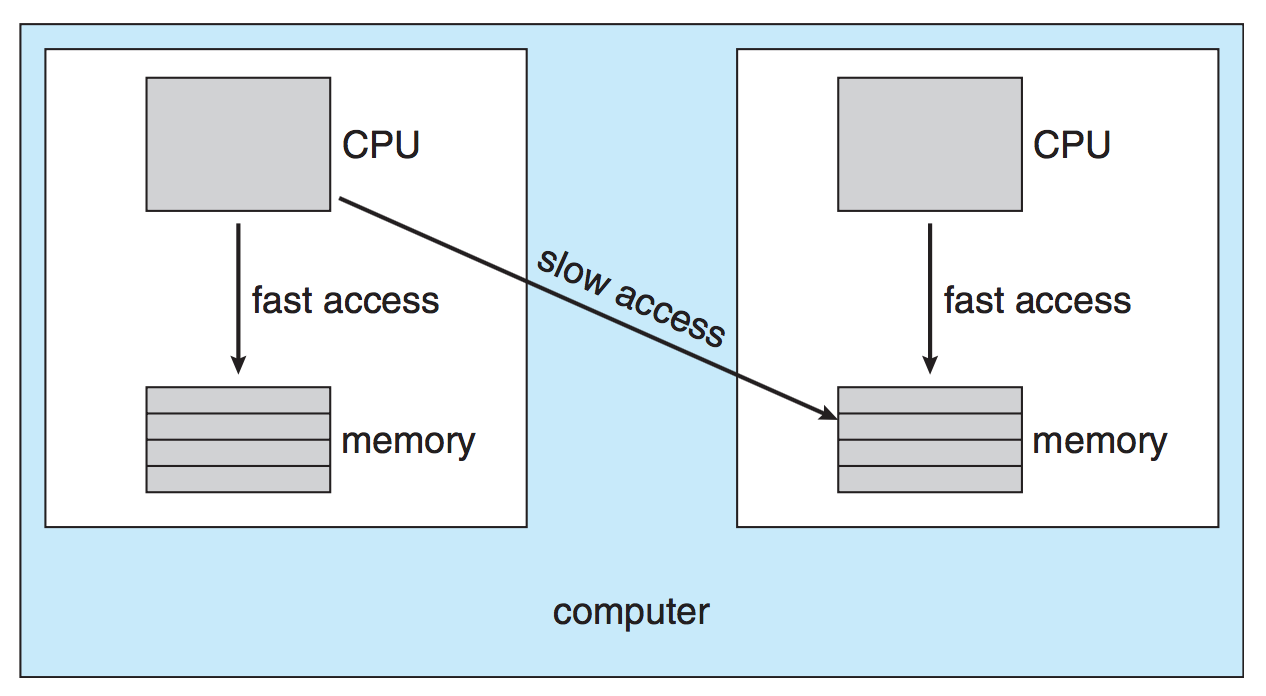
\includegraphics[width=0.5\textwidth]{images/numa.png}\\
	A system with Non-Uniform Memory Access (NUMA) times~\cite{osc}.
\end{center}

If we have this situation, then our choice of processor should be based on where the memory of the process is located. The memory allocation routine should also pay attention to where to allocate memory requests, preferring to keep the program code together in memory. If there is data in one of the other blocks of memory, it does not mean game over, but it means slower execution.

\subsection*{Load Balancing}
It is presumably obvious that if we have 4 processors, it is less than ideal to have one processor at 100\% utilization and 3 processors sitting around doing nothing. We want to keep the workload balanced between all the different systems. The process for this is \textit{load balancing}.

Load balancing is typically necessary only where each processor has its own private queue of processes to run (the ``grocery store queue'' model); if there is a common ready queue (the ``bank queue'' model) then load balancing will tend to happen all on its own, as a processor with nothing to do will simply take the next process from the queue. But in most of the modern operating systems we are familiar with, each processor does have a private queue, so we need to do load balancing~\cite{osc}.

There are two, non-exclusive approaches to redistributing the load: \textit{push} and \textit{pull} migration. It is called migration because a process migrates from one processor to another (it moves homes). If there is push migration, a task periodically checks how busy each processor is and then moves processes around to balance things out (to within some tolerance). Pull migration is when a processor with nothing to do ``steals'' a process from the queue of a busy processor. The Linux and FreeBSD schedulers, for example, use both~\cite{osc}.

Load balancing, as you can imagine, sometimes conflicts with processor affinity. If a process has a hard affinity for a processor, it cannot be migrated from one processor to another. If there is a soft affinity, it can be moved, but it is presumably not our first choice and we will move that process only if we have no other option. Even then, we might consider what to do: should we always move a process despite the fact that it means a whole bunch of cache misses? Should we never do so and leave processors idle? Perhaps the best thing to do is to put a certain ``penalty'' on moving and only move a process from one queue to another if it would be worthwhile (i.e., the imbalance is sufficiently large).

\subsection*{Multicore Processors}
Before the early 2000s, the only way to get multiple processors in the system was to have multiple physical chips. But if you open up your laptop you are likely to find one physical chip. What gives? \textit{Multicore processors}. As far as the operating system is concerned, a quad-core chip is made of four logical processors, but it's all in one package and this can be faster and more convenient.

When a processor issues a memory read or write that is a cache miss (so the read has to go to memory), the CPU core can spend a lot of time (perhaps as much as 50\%) of its time waiting for that read to take place. We might refer to periods of time where there is computation as a compute cycle, and time spent waiting for memory as a \textit{memory stall}. These tend to alternate, though the length of time for each will vary significantly. It's all a question of how often memory is accessed and how many cache misses there are. See the diagram below:

\begin{center}
	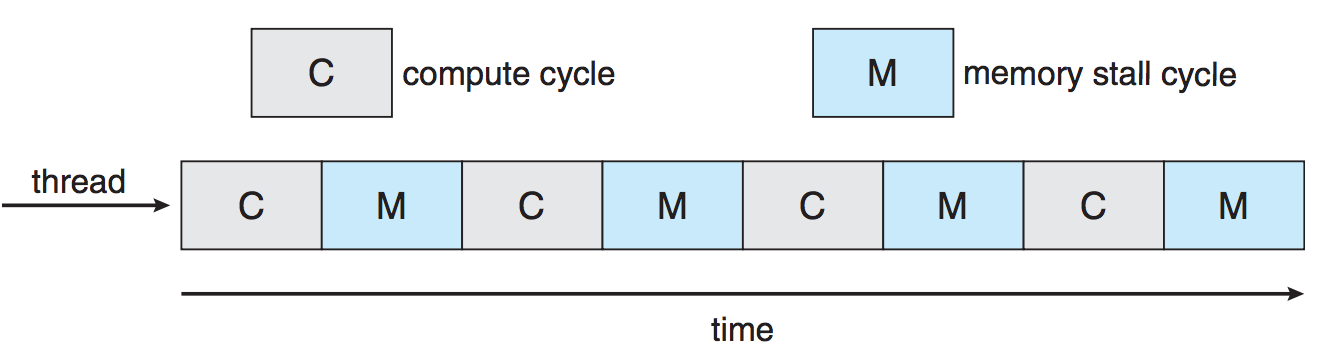
\includegraphics[width=0.7\textwidth]{images/memory-stall.png}\\
	Alternating compute and memory stall cycles~\cite{osc}.
\end{center}

During a memory stall, the processor core may have nothing to do. As you might learn about if you take a course in processor design or programming for performance, you can sometimes move instructions around so that the memory read goes out ``early'' and a few other instructions can be executed in the meantime. 

To offset this problem, the solution was originally called \textit{hyperthreading}: two threads are assigned to each core; if one thread does a memory access or stalls, the code can switch to another thread with a limited penalty. The first CPU I had with hyperthreading was a Pentium IV (it was 2003), and it had one physical core but it would seemingly work on two threads at a time. See below:

\begin{center}
	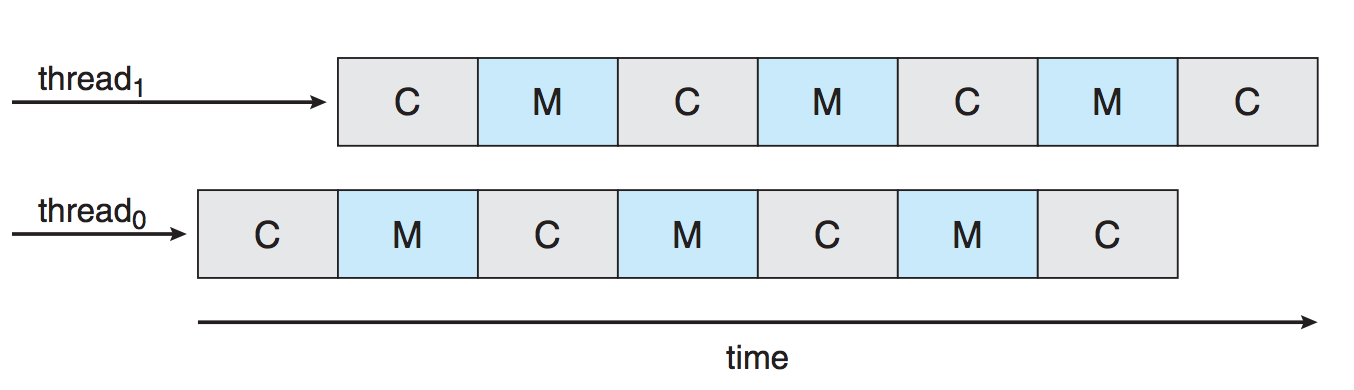
\includegraphics[width=0.7\textwidth]{images/hyperthreading.png}\\
	Hyper threading in a single CPU core~\cite{osc}.
\end{center}

If we have coarse-grained multithreading, a thread will execute for a while and when there is a memory stall (or some other reason why a process gets blocked) then the processor will swap to another thread or process, flushing the instruction pipeline. That is expensive. If we have fine-grained multithreading, it looks more like the diagram above where we have alternation between two threads that are in the pipeline at the same time. The cost of switching between these two threads is small~\cite{osc}.

So now we have two different levels of scheduling: assigning a process or thread to a processor (the job of the operating system) and deciding when to swap between the two threads in the core (typically the job of the hardware). 




\bibliographystyle{alphaurl}
\bibliography{350}


\end{document}